\section{Method}
\label{sec:method}

\begin{figure}
	\centering
	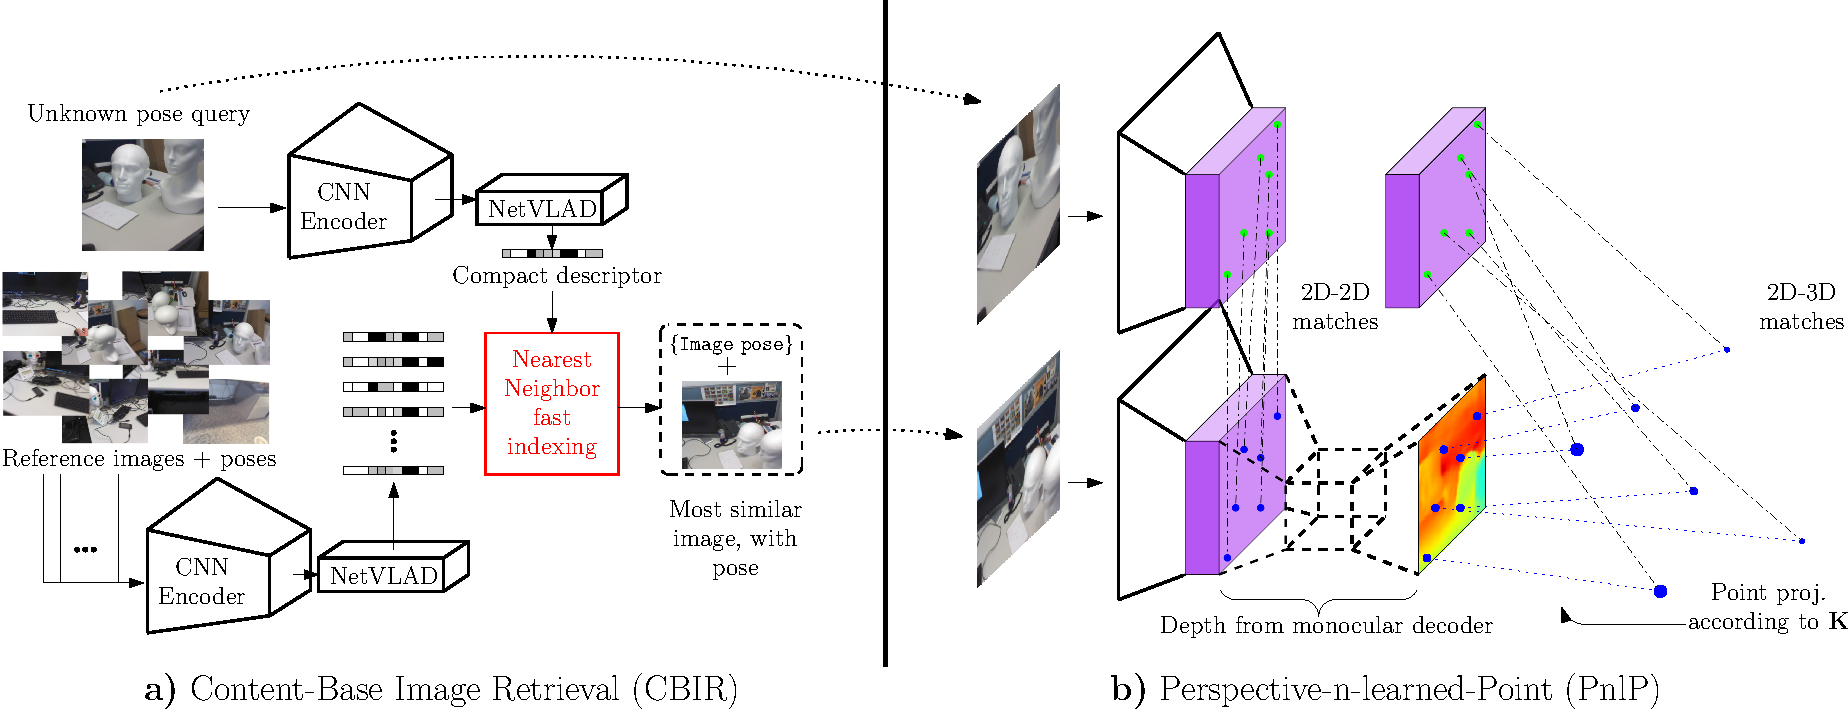
\includegraphics[width=\linewidth]{method/pipeline}	
	\caption[Pipeline of our pose refinement method]{\label{fig:pipeline} Pipeline of the proposed method. \textbf{a)} We retrieve initial pose of an image query using CBIR. \textbf{b)} We refine initial pose with a PnP algorithm where 2D to 3D matches are obtained through the reconstructed depth map of the reference image. \textcolor{purple}{Purple boxes} are deep features blocks used for dense images matching.}
\end{figure}

The camera pose is estimated following this four-step algorithm:
\begin{enumerate}
	\item we obtain the initial pose of the query image by \ac{cbir} (section~\ref{subsec:image_indexing}),
	\item then we finding dense correspondences between the query image and the best retrieved images (section~\ref{subsec:matching}).,
	\item meanwhile, we use a neural network to create the depth map related to the images (section~\ref{subsec:depth_map}),
	\item finally, we use the dense correspondences as well as the reconstructed depth maps to compute relative poses from the retrieved candidates and the query image, using geometric reasoning (section~\ref{sec:relative_pose}).
\end{enumerate}

The two first steps of our pose refinement method are illustrated in figure~\ref{fig:pipeline}.

\paragraph{Notations.}
The aim of our method is to recover the exact 6~\ac{dof} camera pose $\mathbf{h}^q\in\mathbb{R}^{4\times 4}$, represented by a pose matrix in homogeneous coordinates, corresponding to an input RGB image $x^q\in\mathbb{R}^{3\times H\times W}$. We know the matrix $\mathbf{K}\in\mathbb{R}^{3\times 3}$ of intrinsic parameters of the camera. We assume that we know the pose $\left\{ \mathbf{h}^r_{i} \right\}_{i\in\left[1,N\right]}$ of a pool of $N$ references images $\left\{ x^{r}_i \right\}_{i\in\left[1,N\right]}$ of the scene where we want to localize the query. These poses can be obtained by \ac{sfm} or by using external sensors. We denote as $E$, respectively $D$, a neural network encoder, respectively decoder. $P$ denotes the pooling layer used to create a global image descriptor for image indexing.

\subsection{Image retrieval}
\label{subsec:image_indexing}

\Ac{cbir} for localization are deeply detailed in the previous chapter. We provide a short explanation in the following.  We assume that the reference data are augmented with 6-\ac{dof} pose information and we cast the initial pose estimation task as a \ac{cbir} problem like in~\cite{Balntas2018}. In order to evaluate the similarity between the unknown pose query image $x^q$ and the $N$ reference images $\left\{ x_{i}^r \right\}_{i\in\left[1,N\right]}$, we need to use a discriminative image representation. We use deep global image descriptor for place recognition, to describe the data by low-dimensional $L_2$ normalized vectors. The image descriptor $f(x^q) $ is obtained by concatenating the dense feature from neural network encoder $E$: 
\begin{equation}
	f(x^q) = P(E(x^q)).
\end{equation}
\noindent In the following, we write $f(x^q)$ as $f^q$ for readability.

We first compute reference descriptors $\left\{ f_{i}^r \right\}_{i\in\left[1,N\right]}$ from the reference images. Then we compare the query descriptor $f^q$ to the pre-computed descriptors by nearest neighbour indexing and retrieval:
\begin{equation}
	\left\{ f^{sim}_j \right\}_{j\in\left[1, K\right]} = sim \left( f^q, \left\{ f^r_i\right\}_{i\in\left[1,N\right]} \right),
\end{equation}
where $sim$ is the nearest neighbour matching function and $f^{sim}_j, j \in [1, K]$, the ranked $K$ closest reference descriptors to the query descriptor. We use cosine similarity to evaluate the similarity between two descriptors and K-D tree as indexing structure. We consider poses $\mathbf{h}^{sim}_{j \in [1, K]}$ as initial candidate poses of the image $x^q$.

\subsection{Dense correspondences}
\label{subsec:matching}
In order to refine the initial pose obtained by image retrieval, we compute correspondences between the query image and the closest retrieved image candidates. In~\citep{Taira2018, Noh2017, Widya2018}, authors use the dense features extracted by a convolutional neural network in order to compute correspondences between images. We follow the same idea and use the latent representation already computed by the neural network encoder $E$ to compute correspondences between the query image and the $K$ retrieved candidates. Since we only consider the $K$ nearest neighbours to our query, dense features matching is tractable.

Local image descriptors $d_{l,m}$ are obtained from the latent image representation by concatenating the features at each position $\left( l, m \right)_{W_\mathrm{E},H_\mathrm{E}}$ ($W_\mathrm{E}$ and $H_\mathrm{E}$ are the spatial dimensions of the features map) along the depth of the features map~\citep{Taira2018, Widya2018}. We subsequently $L_2$-normalize the extracted descriptors before matching. We consider only consistence matches by rejecting correspondences that do not respect the bidirectional test (nearest descriptors of image 1 in image 2 have to be the same as nearest descriptors of image 2 to image 1).

\subsection{Depth from monocular image}
\label{subsec:depth_map}
2D to 2D correspondences obtained by dense features matching (section~\ref{subsec:matching}) do not provide enough information to compute relative pose between images at absolute scale. Therefore, we propose to reconstruct the relative scene geometry from the camera to circumvent this limitation. Various recent deep learning generative models are able to properly reconstruct geometry associated to radiometric data, with full supervision training~\cite{Eigen2014}, weakly annotated data~\cite{Godard2017} or even in a self-supervized way~\cite{Mahjourian2018}. 

We train an encoder/decoder jointly to predict the corresponding depth map $\hat{z}$ associated to an image: $\hat{z} = D(E(x))$. With the generated depth map obtained by our neural network and the intrinsic parameters of the camera $\mathbf{K}$, we can project the 2D point $\left( l, m \right)^T$ to the corresponding 3D coordinate $\mathbf{p}$:
\begin{equation}
	\label{eq:3d_proj}
	\mathbf{p} = \hat{z}_{l, m} \cdot \mathbf{K}^{-1}[l, m, 1]^T.
\end{equation}